\documentclass{standalone} \usepackage{tikz} \usetikzlibrary{patterns,calc}
\def\centerarc[#1](#2)(#3:#4:#5)[#6](#7){ 
	\draw[#1] ($(#2)+({#5*cos(#3)},{#5*sin(#3)})$) arc (#3:#4:#5) node[#6]{#7}; }
\begin{document}
	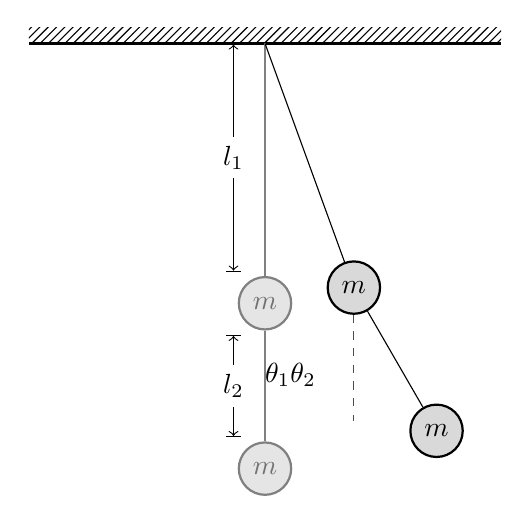
\begin{tikzpicture}
	\node[circle,draw=black!50,thick,fill=black!10,
	minimum width=6mm,minimum height=6mm,text opacity=0.5] (A) at (0,1.0) {$m$};
	\node[circle,draw=black!50,thick,fill=black!10,
	minimum width=6mm,minimum height=6mm,text opacity=0.5] (A') at (0,-1.1) {$m$};
	\fill [pattern = north east lines] (-3,4.3) rectangle (3,4.5);
	\draw[thick] (-3,4.3) -- (3,4.3);
	\draw[draw=black!50] (0,4.3) -- (A);	\draw[draw=black!50] (A) -- (A');
	\draw[|<->|] (-0.4,4.3) -- (-0.4,1.4) node[pos=0.5,fill=white]{$l_1$};
	\draw[|<->|] (-0.4,0.6) -- (-0.4,-0.7)
	node[pos=0.5,fill=white]{$l_2$};
	\begin{scope}[rotate around={20:(0,4.3)}]
	\node[circle,draw=black,thick,fill=black!15,minimum width=6mm,minimum height=6mm,text opacity=1] 
	(B) at (0,1.0) {$m$};
	\draw[draw=black] (0,4.3) -- (B);
	\begin{scope}[rotate around={10:(B)}]
	\node[circle,draw=black,thick,fill=black!15,minimum width=6mm,minimum height=6mm,text opacity=1] 
	(B') at (0,-1.1) {$m$};
	\draw[draw=black] (B) -- (B');
	\end{scope}	
	\end{scope}
	\draw[dashed,draw=black!70] (B) -- +(0,-1.7);
	\centerarc[](0,4.3)(-90:-90+20:1.3)[below,midway]($\theta_1$)
	\centerarc[](B)(-90:-90+30:1)[below,midway]($\theta_2$)
	\end{tikzpicture}
\end{document}
